% SPDX-License-Identifier: Apache-2.0
\documentclass[11pt,letterpaper]{article}
\usepackage[margin=0.78in,headheight=16pt]{geometry}
\usepackage[T1]{fontenc}
\usepackage{lmodern,microtype,amsmath,amssymb,graphicx,booktabs,longtable,array,xcolor}
\usepackage[most]{tcolorbox}
\usepackage{enumitem,fancyhdr,titlesec,caption,float,needspace}
\usepackage[colorlinks=true,linkcolor=teal,citecolor=teal,urlcolor=teal,breaklinks=true]{hyperref}
\usepackage{xurl}
\definecolor{ink}{HTML}{142B3A}
\definecolor{teal}{HTML}{087E8B}
\definecolor{coral}{HTML}{C85B45}
\definecolor{pale}{HTML}{EFF6F6}
\definecolor{muted}{HTML}{506273}
\hypersetup{pdftitle={AGI ALPHA FLYWHEEL: When Capability Creates Opportunity},pdfauthor={Vincent Boucher, President of MONTREAL.AI}}
\setlength{\parindent}{0pt}
\setlength{\parskip}{6.5pt}
\setlength{\emergencystretch}{2em}
\widowpenalty=10000
\clubpenalty=10000
\setlist{nosep,leftmargin=1.3em}
\titleformat{\section}{\large\sffamily\bfseries\color{ink}}{\thesection}{0.65em}{}
\titleformat{\subsection}{\normalsize\sffamily\bfseries\color{teal}}{\thesubsection}{0.65em}{}
\captionsetup{font=small,labelfont=bf}
\pagestyle{fancy}
\fancyhf{}
\fancyhead[L]{\small\sffamily AGI ALPHA FLYWHEEL}
\fancyhead[R]{\small\sffamily Research edition \textbar{} 27 October 2026}
\fancyfoot[L]{\small\sffamily Vincent Boucher \textbar{} MONTREAL.AI}
\fancyfoot[R]{\small\sffamily\thepage}
\renewcommand{\headrulewidth}{0.3pt}
\newtcolorbox{findingbox}[1]{colback=pale,colframe=teal,boxrule=0.5pt,arc=2pt,title=#1,fonttitle=\sffamily\bfseries,breakable}
\newcommand{\artifact}[1]{\texttt{\small #1}}
\newcommand{\money}[1]{\$#1}
% Generated from recorded results; no model outputs are assumed here.

\begin{document}
\begin{titlepage}
\vspace*{0.12in}
{\color{teal}\sffamily\bfseries\large AGI ALPHA FLYWHEEL}\par
\vspace{0.23in}
{\sffamily\bfseries\color{ink}\fontsize{32}{36}\selectfont WHEN CAPABILITY\\CREATES OPPORTUNITY}\par
\vspace{0.17in}
{\Large Transformational Intelligence, Experience-Trained Specialists\\[3pt] and the Expanding Frontier of Profitable Work}\par
\vspace{0.22in}
{\large\bfseries Vincent Boucher}\par
{\large President of MONTREAL.AI}\par
\vspace{0.16in}
{\sffamily\color{teal} FIND YOUR ALPHA. BUILD YOUR SUCCESSOR $\Omega$.}\par
\vspace{0.17in}
\begin{findingbox}{What this edition establishes}
\small
\textbf{A real but conditional transfer effect.} On 24 unfamiliar compatible response functions, v2 produced 21 accepted models inside a 24-call candidate budget; the strongest ordinary model arm produced one. In the separately frozen compound mission, v2 delivered 17 of 24 checked plans with 40 total queries, versus seven for the strongest individual conventional arm. A marketed response model also pays for 384 independent acceptance observations. Every accepted compound plan includes sixteen measured context checks. Shift, stronger budgets and simple direct solutions narrow the advantage. The primary economic policy rejects optional learning; no customer revenue or sustained compounding is established.

\end{findingbox}
\vspace{0.12in}
\begingroup\small
\textbf{Abstract.} A useful agent enterprise can profit from competent delivery before retaining any skill. The additional research question is whether productive experience leaves an advantage that survives strong ordinary methods, independent acceptance and complete accounting. We execute a bounded scientific-software experiment: an originating characterization job learns an empirical interaction prior; optional practice expands it; fresh recipients reuse its actual bytes to fit unfamiliar response functions and propose operating decisions. We compare ordinary sparse regression, adaptive experiment design, direct decision search, the original artifact, the developed artifact, an unrelated artifact and an ordinary library containing identical information. The simulator family and learning procedure are researcher constructed; its mathematical structure, updates, transfer and output checks execute. Demand, selling prices, simulator tariffs, frontier-model token use and collections are explicitly conditional scenarios. We charge operational verification, preserve distribution shift and failed investments, and distinguish research evaluation from customer delivery. The result is a causal, reproducible account of where reusable empirical structure helps, where strong alternatives erase the advantage, and why neither a useful artifact nor simulated profit establishes a self-accelerating enterprise. A protected research transfer reuses the existing AGI ALPHA lifecycle without claiming live ENS authentication or extending production execution authority.\par
\endgroup
\vfill
{\small\color{muted} Research cut: 27 October 2026. Starting repository source: \texttt{80b345828f34fd8a6e592977dd17ef37141305f4}.\\Observed customer collections: \money{0}. No live frontier benchmark, physical-engineering validation, customer trial or production ENS authentication is claimed.}
\end{titlepage}
\setcounter{page}{2}

\section{A useful outcome before a flywheel claim}

Consider a scientific-software owner who can run an expensive simulator but does not yet know which combinations of inputs produce a useful operating point. The customer needs an executable model, a verified decision or a diagnosis they can act on. A smaller regression error matters only if it changes one of those deliverables. The central opportunity is therefore to preserve what previous work reveals about a problem family, while testing whether that knowledge removes a consequential bottleneck on new work.

This study deliberately distinguishes five claims. \emph{Commercial delivery} means that an accepted outcome sells above complete cost. \emph{Specialist development} means that retained experience improves fresh work beyond the recipient's competent current methods. \emph{Network value} means that sharing adds more benefit than its additional costs. \emph{Productive expansion} means that an otherwise fixed useful offering becomes deliverable inside its declared quality, cost and deadline envelope. \emph{Sustained compounding} requires successive improvements beyond additional resources, workload or model upgrades. None follows automatically from the preceding claim.

\begin{center}\small\begin{tabular}{p{0.26\linewidth}p{0.65\linewidth}}
\toprule
Question & Evidence in this edition \\ \midrule
Commercial delivery & Positive conditional simulations; actual sales = 0 \\
Specialist development & Fresh sparse-representation transfer is observed \\
Network value & Actual fixture transfer; same-content library parity \\
Productive expansion & Scoped 40-query compound-outcome crossings \\
Sustained compounding & Not established by this one-development-cycle study \\
\bottomrule
\end{tabular}\end{center}


The strongest measured claim is intentionally narrower than ``frontier intelligence has reached a limit.'' Our executable Beta portfolio represents capable conventional tools that a competent frontier agent could use. We did not benchmark a live tool-using Astra or Terra agent on these tasks. The broader frontier-model comparison remains a commissioning experiment. The paper reports an empirical mechanism, its costs and its failure boundaries rather than assigning superiority to an agent label.

\section{What changed after the previous experiments}

The study starts from actual source and result files rather than earlier mission statements. The source audit preserves the thermal study at \texttt{71d1054} and the scheduling study at \texttt{79948bc}; full identities and file hashes are in the companion. The thermal work improved approximation error substantially, yet both raw transferred approximations failed all 64 acceptance checks. Correcting the output recovered usefulness, but an ordinary spectral-preconditioned method left only approximately 0.125 milliseconds of average v2 saving in the reported transfer comparison. A simple ordinary router nearly matched the specialist, and shifted tasks could make it worse. The scheduling study's learned dispatcher was likewise challenged by a stronger conventional search: the reported fresh comparison against Beta144 reversed the nominal and robust advantage. These are source-specific historical observations, not recomputed results of this edition.

Those outcomes identify three bottlenecks. First, numerical improvement can be a proxy for an outcome the customer still cannot accept. Second, known algorithms can absorb most of the apparent advantage once the baseline has a competent search budget. Third, a very small saving may be commercially irrelevant after assessment, maintenance and correction. None of these findings disproves profitable delivery against human-service prices. They restrict what can count as additional Alpha.

We therefore move the unit of investigation from local solver milliseconds to the number of observations needed to produce a checked scientific-software output. Conventional sparse polynomial approximation and support-adaptive experimental design are established methods \cite{diaz,tropp,ard}. Reusing an empirically learned support is not a new regression algorithm. The candidate advantage is the information preserved from earlier jobs, and the decisive questions are whether that information transfers, whether its absence causes the difference, and whether obtaining and maintaining it was worthwhile.

\section{Define the productive frontier precisely}

Let an offering $o$ specify a beneficiary, a complete deliverable, acceptance rule $Q_o$, deadline $D_o$, customer effort bound $E_o$, price $p_o$ and admissible operating conditions $\mathcal{X}_o$. Let $\pi$ be an execution and investment policy, and $K$ the available resources. Its productive frontier is
\[
\mathcal{F}_{\pi}(K)=\{o:\Pr(Q_o=1\mid\pi,\mathcal{X}_o)\geq q_o,\;
T_o\leq D_o,\;E_o^{\rm actual}\leq E_o,\;
\mathbb{E}[p_o^{\rm collected}-C_o^{\rm complete}]>0\}.
\]
Here $q_o$ is an agreed reliability requirement, not a label applied after seeing results. Customer demand and collection must be credible in addition to technical acceptance. A small synthetic sample can estimate a conditional acceptance rate, but cannot establish the real-market set $\mathcal{F}_{\pi}$.

We report a finite \emph{experimental} frontier: the number of generated tasks whose fixed output requirements a method meets inside each declared query budget. Where economics are attached, the result is conditional on explicitly stated tariffs, prices and buyer behavior. If both configurations qualify at the same scope and budget, the outcome is better economics or higher reliability, not newly feasible work. If Beta qualifies after additional calls, the crossing is relative to the smaller declared envelope, not a general impossibility result.

For a candidate artifact $s$, expected incremental net value at decision time $t$ is
\[
\widehat{V}_{t}(s)=\sum_{j>t}\widehat{\Pr}_{t}(\text{eligible reuse }j)
\widehat{\Delta b}_{t,j}(s)-\widehat{C}_{t}^{\rm assess,retain,share,serve,maintain,requalify}(s).
\]
The estimate uses only then-available development evidence. We retain the admission errors and costs. ``Alpha'' describes positive net mission advantage over the recipient's current Beta; it is not a permanent property of a file. If an ordinary library already exposes the same information and execution behavior, that capability belongs in Beta.

\section{Opportunity portfolio and independent reasons to care}

Three primary offerings share a potential information bottleneck while asking different questions of the output. After development exposed a cheaper direct solution to the single-plan mission, a separately frozen extension proposed a fourth, more demanding outcome: one operating plan checked across sixteen environmental contexts.

\begin{longtable}{p{0.19\linewidth}p{0.35\linewidth}p{0.37\linewidth}}
\toprule
Offering & Beneficiary and complete output & Failure condition \\
\midrule
Response characterization & A scientific-software owner receives an executable response model, its domain, fresh prediction report, dependencies and reproducible observations. & Strong ordinary methods reach equivalent fresh accuracy at equal complete cost; verification consumes the saving; the learned family assumption fails. \\
Verified inverse design & A design engineer receives a concrete input vector from a fixed feasible menu, its known input cost and a newly measured simulator response meeting the frozen specification. & The final simulator measurement fails, input cost exceeds the fixed ceiling, or ordinary direct search meets the same condition as economically. \\
Fault diagnosis prototype & A maintenance engineer receives a proposed changed interaction and an explanation checked against additional diagnostic observations; deployed repair is outside scope. & A simpler paired old/new measurement method resolves the fault; the diagnosis is incorrect; the old model's error overwhelms the change. \\
Robust operating plan (supplement) & A design engineer receives one control vector and sixteen newly measured environmental responses satisfying a fixed aggregate and coverage requirement. & Ordinary search meets the same complete query budget; context verification erases savings; the shared representation fails under shift. \\
\bottomrule
\end{longtable}

Scientific-software and algorithm-development consulting is an offered external service. SDSU's CSRC lists an external rate of \money{80} per hour; Purdue lists an industry research-software consulting range of \money{26}--\money{115}; ParaTools publishes a much higher senior-specialist rate. Objective Experiments lists a custom experiment design at \money{500} and consultation at \money{300} per hour \cite{sdsu,purdue,paratools,objective}. These sources support a plausible purchasing category and rate anchors. They do not establish the number of customers, matched project hours, demand for this implementation or willingness to pay for an autonomous service.

The economic scenarios therefore mark human hours as assumptions and estimate reference prices by multiplying hours by a sourced external rate. A new diagnostic product without a comparable complete human service receives a willingness-to-pay hypothesis, not a purported market price. Buyer choices include purchasing, choosing a human alternative, deferring and declining. The first operational step is a scope-matched customer pilot, not extrapolation from a synthetic acceptance table.

The proposed reuse boundary is a customer's recurring simulator family with a stable interface and feature convention, rather than all scientific work. Human delivery requires understanding the input domain, building a callable experiment harness, choosing and revising experiments, diagnosing numerical failures and packaging an independently checkable result. The assumed twelve-hour model and sixteen-hour design scopes cover this whole engagement; no measured human time study supports those durations. A competent frontier agent can automate much of that workflow, but must still obtain observations of an unknown black-box response. The candidate specialist targets that observation bottleneck. Whether a real Astra-class agent can discover an equally good representation on demand is unmeasured, and is a specific falsification test for the next pilot.

The diagnostic case reuses a nominal response model across maintenance incidents, but availability of the original simulator makes a paired conventional experiment decisive. The compound-plan case reuses interaction structure across changing coefficients and environmental contexts; it is consequential only when querying the real system is expensive enough, the finite-context specification is useful, and family qualification does not consume the saved resources. No evidence here establishes a plausible volume of compatible buyers. The simulated four arrivals per day is a workload stress assumption, not a market forecast.

\Needspace{8\baselineskip}
\section{Executable learning and protected fresh evaluation}

\subsection{A transparent scientific-response environment}

The environment is a deterministic, ten-input polynomial response family over bounded inputs, represented in a known total-degree-three Legendre library with 286 terms. Each task has a sparse active set; compatible tasks draw their interactions from a recurring family, partial shifts introduce unfamiliar interactions, and novel-family tasks move outside the learned family. The generator is a researcher-authored test bed. It is not a calibrated thermal, aerospace or manufacturing simulator, and its normalized response units are not physical units.

All methods know the generic feature library. They do not receive the current task's hidden coefficients or support. A learner obtains responses by querying points, pays for its visible validation observations and refits coefficients for the new task. Thus the inherited artifact stores which interactions earlier work found useful, not the answers to new tasks. No pretrained proprietary model weights are modified.

\subsection{Origin, optional Gym and distinct recipients}

The originating job learns a model using ordinary sparse regression and retains v1's observed support. The optional Gym repeats the same automatic update on additional diverse jobs. The resulting v2 stores empirical support frequencies and a versioned union. A recipient fits new numerical coefficients using that representation. A validation guard can reject an incompatible prior and compare with the ordinary portfolio. The origin, v1, Gym events, v2, recipient observations and delivered outputs are retained as machine-readable artifacts.

The originating fit consumed 128 observations and 384 separately paid response-accuracy checks. It retained nine terms, including the intercept. Ten optional Gym jobs consumed 1,280 additional fitting observations. Each fitted job retained 9--9 nonzero terms; their empirical union contains 21 terms. All eleven research characterization fits met the fresh prediction criterion. Those successful fits are not themselves evidence that retention repays its assessment cost. The primary confirmation contains 48 unfamiliar tasks and 1,728 method--budget rows; the independent compound extension adds 48 further tasks and 1,728 rows.


This is actual experience-dependent algorithmic learning: the artifact bytes are computed from observations and change the subsequent fitted model. The feature library, update mechanism, task generator and software are researcher authored with AI assistance. There is no claim that an autonomous enterprise invented sparse regression or independently discovered an engineering law. The experience-driven aims described by Ineffable Intelligence motivate the question; they are neither evidence for these results nor an affiliation \cite{ineffable}.

\begin{figure}[H]
\centering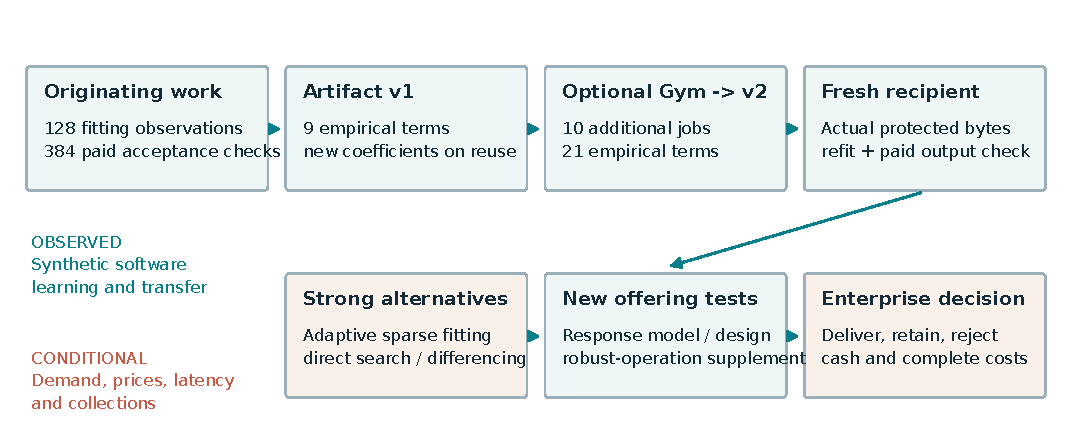
\includegraphics[width=\linewidth]{figures/lineage.pdf}
\caption{Capability lineage and evidence boundaries. The measured path is an executable empirical representation, its protected transfer and fresh refitting. Commercial quantities and live commissioning remain separately identified.}
\end{figure}

\subsection{Strong baseline portfolio and causal controls}

The conventional portfolio includes validation-selected orthogonal matching pursuit, automatic relevance determination and ridge regression. Experiment designs include space filling, a pivoted-QR approximation to D-optimal selection and a pilot fit followed by support-adaptive augmentation. The adaptive variant matters because prior literature already exploits estimated support to select informative experiments \cite{diaz}. A direct operating-plan search can bypass model construction altogether when the customer only needs a satisfactory decision.

The causal arms are v1, v2, an unrelated prior and an oracle-informed diagnostic comparator. The oracle receives support information unavailable to an operational policy but still uses the constrained fitting procedure, so it is not a mathematical upper bound. An ordinary-library arm uses exactly the v2 information and the same permitted computation. That control prevents a graph or network label from receiving credit for information that a simpler library serves equally well. An ex-post best-Beta envelope is reported only as a deliberately generous diagnostic, never as an implementable clairvoyant policy.

Training, development and confirmation seeds are disjoint. Development chooses policies before confirmation. Source, protocol and learned artifacts are hashed at the freeze. The learner's interface receives queried data and allowed artifacts; hidden values belong to the scorer. This is procedural separation within a reproducible research process, not a claim of an adversarially isolated scoring service. A reader can inspect the full generator after the study; the freeze supplies an audit trail, not proof of preregistration with an external authority.

The declared primary research budget was one representation family, one originating job, ten additional Gym jobs, twelve development tasks and forty-eight confirmation tasks, each tested at four budgets. Exactly one subsequent compound-offering extension received its own twelve-task development and forty-eight-task confirmation allowance. We report the earlier constructor and smoke executions as additional research rather than deleting them. This edition stops after that extension; it does not continue searching until a favorable market or task distribution appears.

\subsection{Acceptance that does not hide its cost}

Prediction accuracy uses fresh held-out evaluations and is a separate scientific audit. A commercially offered independently verified response model must pay for those verification observations. The operating-decision offering instead has an immediately observable contract: bounded feasible inputs, a fixed cost ceiling and a fixed response threshold. A final fresh simulator query checks the submitted plan and is charged to that job. Full-menu optimum and regret remain research diagnostics unless a customer explicitly purchases that more expensive guarantee.

Some generated tasks may not contain an acceptable plan in the declared menu. Those cases remain in the denominator; the study does not delete them to manufacture an advantage. The diagnostic prototype likewise pays for its extra probes and independent validation. If access to both old and new simulators permits ordinary paired differencing, it must be treated as a serious alternative rather than pretending the old response is unavailable.

The frozen documents retain two textual inconsistencies rather than silently rewriting history. Earlier portfolio prose described a lowest-cost plan and a regret criterion; the final operational evaluator and acceptance specification require a satisfactory feasible plan, with regret reported separately. One economic deliverable description also over-specified a fitted response model, although the direct-search comparator returns a checked plan and replayable search instead. Explicit companion clarifications identify those discrepancies. All claims here use the implemented feasibility contract, and an accurate response model remains a separate offering.

\section{Experiment A: fresh transfer and the cause of the gain}

The first experiment compares the original v1 artifact, Gym-developed v2 and conventional tools on unseen response functions. It then uses the resulting model to make a different recipient's operating decision, and probes a maintenance diagnosis. The recipient labels are simulated identities; they do not establish live ENS ownership. A transfer is materially useful only if it changes fresh accepted output, and a numerical model improvement can coexist with an unchanged design-decision outcome.

\begin{center}\small\begin{tabular}{lrrrr}
\toprule
Method & 24 & 40 & 64 & 96 \\ \midrule
Beta: space filling & 0/3 & 20/24 & 34/37 & 47/44 \\
Beta: D-optimal & 0/1 & 21/24 & 43/40 & 48/44 \\
Beta: adaptive & 1/6 & 12/17 & 37/39 & 47/44 \\
Beta: direct search & 0/27 & 0/32 & 0/40 & 0/44 \\
Origin v1 & 0/5 & 16/19 & 32/39 & 47/44 \\
Gym v2 & 21/22 & 34/33 & 42/42 & 47/44 \\
Identical-content library & 21/22 & 34/33 & 42/42 & 47/44 \\
Unrelated prior & 0/2 & 18/22 & 35/37 & 48/44 \\
Oracle support & 48/44 & 48/44 & 48/44 & 48/44 \\
\bottomrule
\end{tabular}\end{center}
Each cell is \emph{accepted response models / accepted operating plans}, each out of 48 tasks. A response model additionally requires 384 independent acceptance observations; the plan's final check is inside the displayed budget. Direct search has no response-model deliverable, so its prediction entry is zero. At 24 queries the compatible-family prediction comparison is v2 21/24 versus adaptive Beta 1/24; v1 and the unrelated prior each score 0/24. Across all families, v2's fresh prediction advantage over the ex-post best ordinary arm is 20 wins and zero losses. Its corresponding operating-plan result is six wins and twelve losses: the positive model effect does not imply a positive action effect. At 96 queries D-optimal Beta accepts 48/48 models, versus v2 47/48. Both accept 44/48 operating plans; four menus have no qualifying plan.\par The identical-content library matches v2 on all 192 task--budget pairs. This is evidence that the effective learned information transfers, and evidence against attributing an additional benefit to the graph representation. Partial and novel families preserve negative transfer: at 40 queries, for example, partial-shift v2 model acceptance is 3/12, versus 7/12 for space-filling Beta.


\begin{figure}[H]
\centering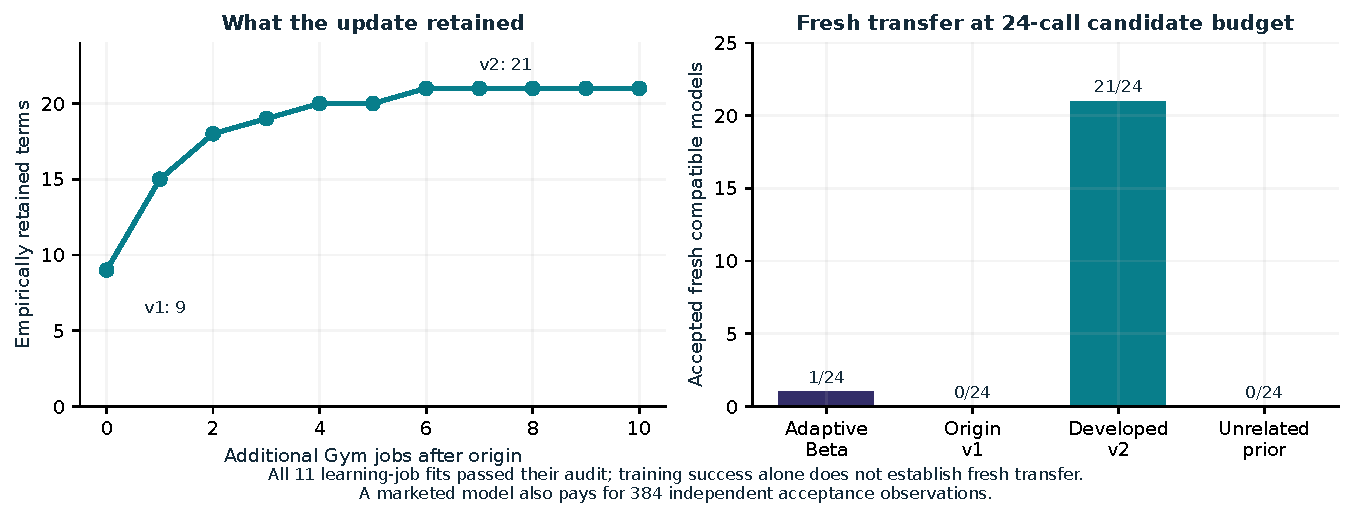
\includegraphics[width=\linewidth]{figures/learning-progress.pdf}
\caption{Learning and fresh performance are separate evidence. The retained union grows from observations; the unfamiliar-task comparison tests whether those retained terms matter. No protected confirmation labels enter the update.}
\end{figure}

\begin{figure}[H]
\centering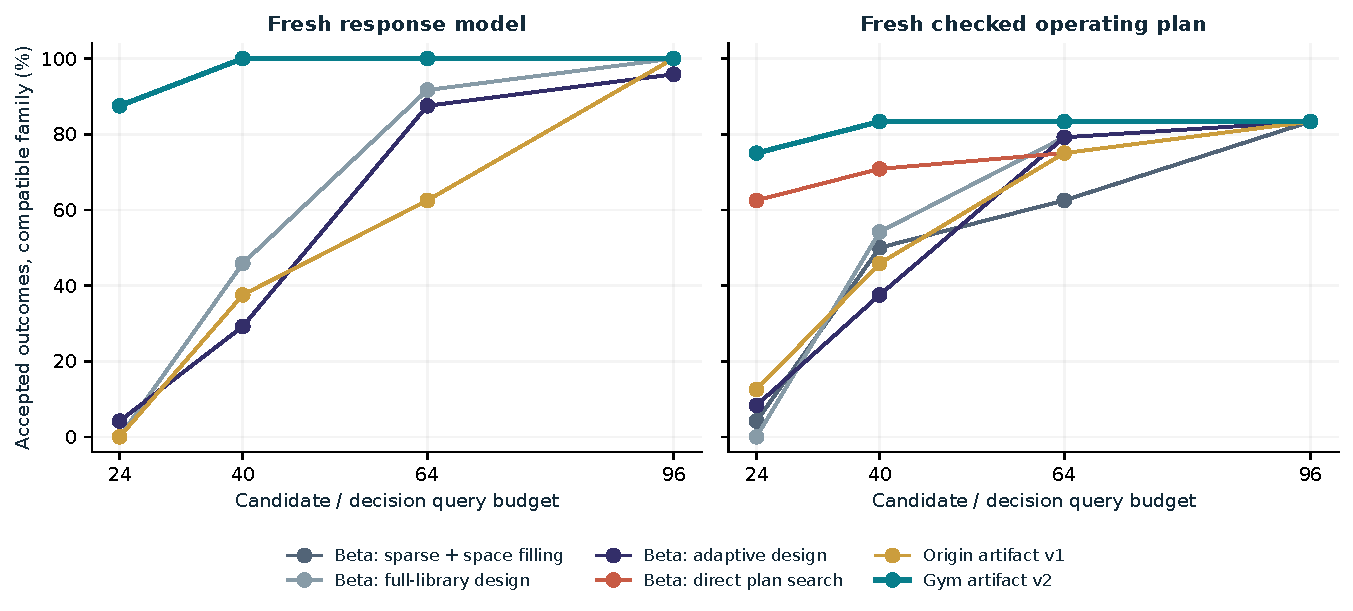
\includegraphics[width=\linewidth]{figures/learning-transfer.pdf}
\caption{Fresh accepted prediction and decision outputs by budget. Each plotted point comes from executed confirmation rows. Predictions and decisions have different acceptance obligations; rates are not interchangeable.}
\end{figure}

\begin{figure}[H]
\centering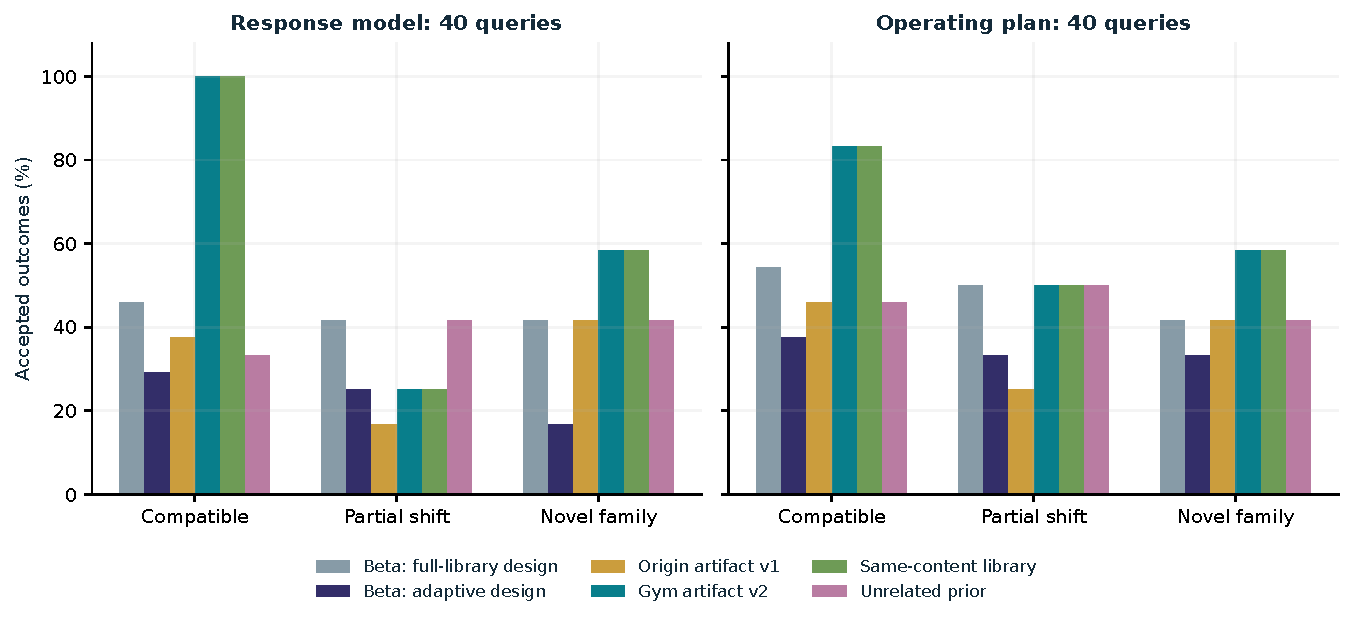
\includegraphics[width=\linewidth]{figures/causal-controls.pdf}
\caption{Causal controls and distribution shift. Same-content library behavior tests the incremental claim for the sharing mechanism; an unrelated prior tests dependence on the inherited information.}
\end{figure}

Sampling uncertainty concerns this generator and these seeds. It does not validate an assumed learning distribution, the fidelity of a physical simulator, a customer's demand or a frontier model's capability. Positive transfer therefore remains conditional on recurring structure and must be requalified when the task family changes.

\section{Experiment B: a fixed-envelope feasibility test}

The second experiment freezes usefulness, a specific output check, query budget and price assumptions before confirmation. For inverse design, the same plan menu, response requirement, input-cost ceiling and paid final verification apply to all configurations. A specialist-only success is a finite-instance feasibility crossing inside that envelope. A pair of successes is an efficiency or reliability comparison. A pair of failures is unresolved or infeasible work; it does not become an offering because the simulator produces a number.

The primary single-plan offering does not establish an overall specialist advantage. At 24 calls, direct search accepts 27/48 operating decisions versus v2 22/48. At 40, the counts are 32/48 and 33/48, but different ordinary arms solve different cases: against the ex-post best conventional envelope, v2 has two unique wins and ten unique losses. Increasing the budget to 96 removes the plan-acceptance difference. These observations preserve commercially useful ordinary delivery while limiting the claim for optional retention.


\begin{figure}[H]
\centering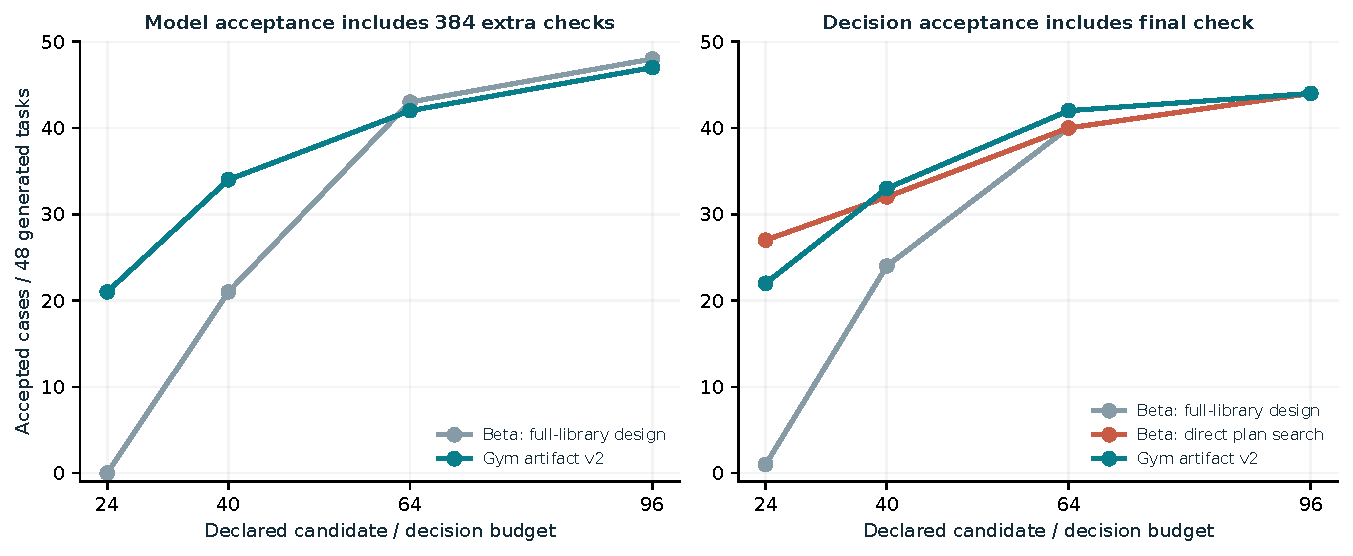
\includegraphics[width=\linewidth]{figures/frontier.pdf}
\caption{The finite experimental productive frontier. This chart counts accepted generated outcomes; it does not estimate the number of real customers or declare a market validated. Larger budgets and stronger conventional methods can close a crossing.}
\end{figure}

The scientific test and the business test are separate. Its synthetic oracle executes cheaply on this machine. Assigning a tariff or latency to a future expensive simulator is a scenario, not a measured invoice or observed deadline. A positive complete-cost scenario supports commissioning that market hypothesis; it does not turn simulated collections into revenue.

\subsection{A stronger offering proposed from the initial experience}

The direct-search result motivated one prospective extension, preserved separately from the primary protocol. The new mission uses the first five simulator inputs as controls and the last five as environmental conditions. One chosen control vector must have mean response at least 0.4 across sixteen fixed contexts, at least twelve nonnegative responses, and known control cost no greater than 1.2. All sixteen final observations are inside the same total budget faced by conventional and retained methods. These normalized thresholds are a declared research specification, not measured buyer requirements.

The direct baseline can reject an unsuitable plan early once five negative responses make the coverage condition impossible, then use remaining calls on another plan. The model baselines may predict across contexts before choosing a control vector, but every accepted output requires all sixteen actual measurements. New development and confirmation seeds, a separate predeclaration and a separate source freeze prevent the original outcome from becoming a silently revised endpoint. The originating artifact is unchanged.

\begin{center}\small\begin{tabular}{lrrrr}
\toprule
Method & 40, compatible & 40, all & 64, all & 96, all \\ \midrule
Beta: space filling & 4/24 & 10/48 & 27/48 & 35/48 \\
Beta: D-optimal & 2/24 & 5/48 & 27/48 & 36/48 \\
Beta: adaptive & 2/24 & 5/48 & 20/48 & 36/48 \\
Beta: direct search & 7/24 & 14/48 & 21/48 & 27/48 \\
Origin v1 & 3/24 & 6/48 & 25/48 & 36/48 \\
Gym v2 & 17/24 & 22/48 & 30/48 & 36/48 \\
Identical-content library & 17/24 & 22/48 & 30/48 & 36/48 \\
Unrelated prior & 7/24 & 11/48 & 24/48 & 35/48 \\
Oracle support & 18/24 & 36/48 & 36/48 & 36/48 \\
\bottomrule
\end{tabular}\end{center}
At 40 total observations, v2 accepts 17/24 compatible-family compound plans; direct search, the strongest individual conventional arm on this stratum, accepts 7/24. The ex-post best of four conventional methods accepts 8/24. In the paired comparison v2 has ten unique wins and one unique loss: +37.5 percentage points, with a conditional task-bootstrap 95 percent interval of +12.5 to +58.3 points. Across all three families, v2 accepts 22/48 and that generous conventional envelope accepts 18/48, with eleven unique wins and seven losses: +8.3 points, interval -8.3 to +25.0 points. The intervals are conditional on the synthetic generator and are not corrected for every exploratory comparison. Thus the strong compatible-family result weakens substantially when recipient structure is unfamiliar. By 96 calls, the strongest conventional model arms and v2 each accept 36/48; twelve menus have no qualifying plan. This is a measured, scoped sample-budget crossing, not proof of universal feasibility or a deployment-grade reliability rate.\par The extension was proposed from development experience and confirmed on new seeds beginning at 1,910,000. Its empirical subpopulation labels are diagnostic: a live enterprise would need an observable family-qualification procedure before using the compatible-family result in a customer promise. Its hypothetical prices and customer demand were not validated or folded into the primary economic ledger.


\begin{figure}[H]
\centering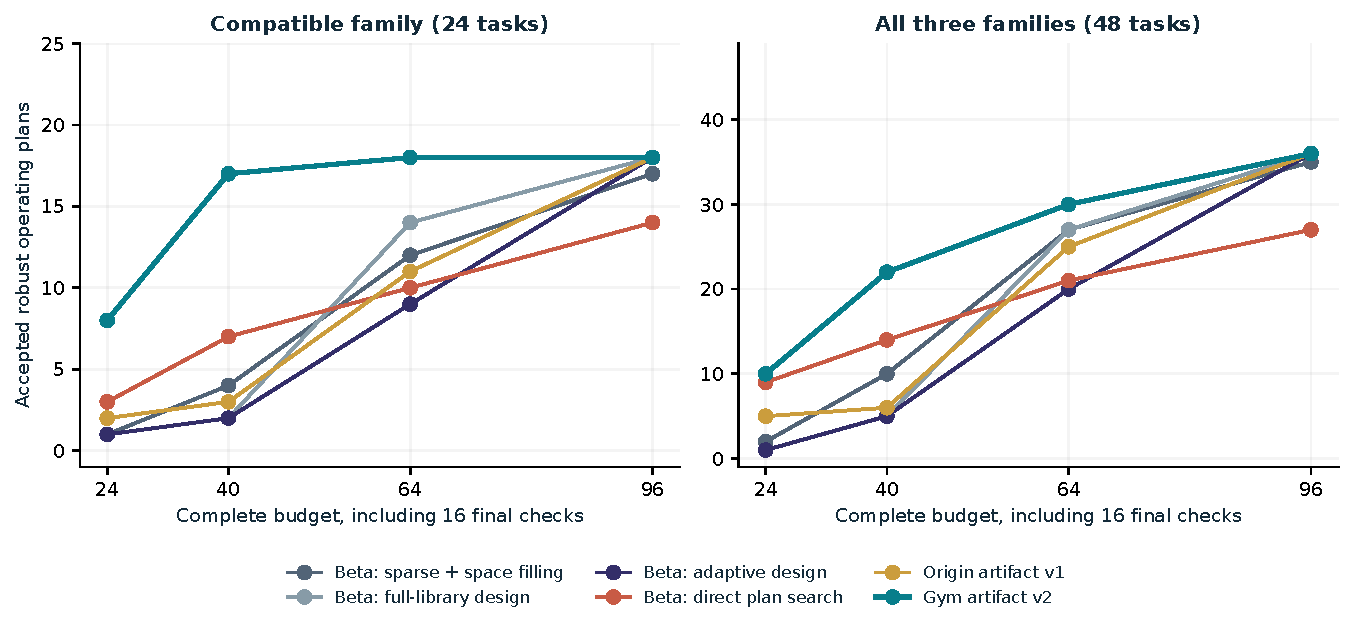
\includegraphics[width=\linewidth]{figures/robust-frontier.pdf}
\caption{The separately frozen compound-outcome experiment. All methods pay for the sixteen final context checks inside each budget. Compatible-family strata diagnose where the mechanism works; their hidden labels are not an operational qualification oracle.}
\end{figure}

\subsection{Inspect one delivered plan and its economic boundary}

The companion exposes every input, coefficient and measured output for task \texttt{robust-1910214}. The v2 recipient uses 40 total queries, including sixteen final context checks, and returns one five-control vector with mean measured response 0.403857, twelve nonnegative responses and known cost 0.906163. Each of the four ordinary configurations fails the same task at the same budget. This task was selected after confirmation as an illustrative crossing; it is already included in the aggregate results and supplies no additional independent replicate. Its small mean margin above 0.4 is not evidence of tolerance to measurement noise.

\begin{figure}[H]
\centering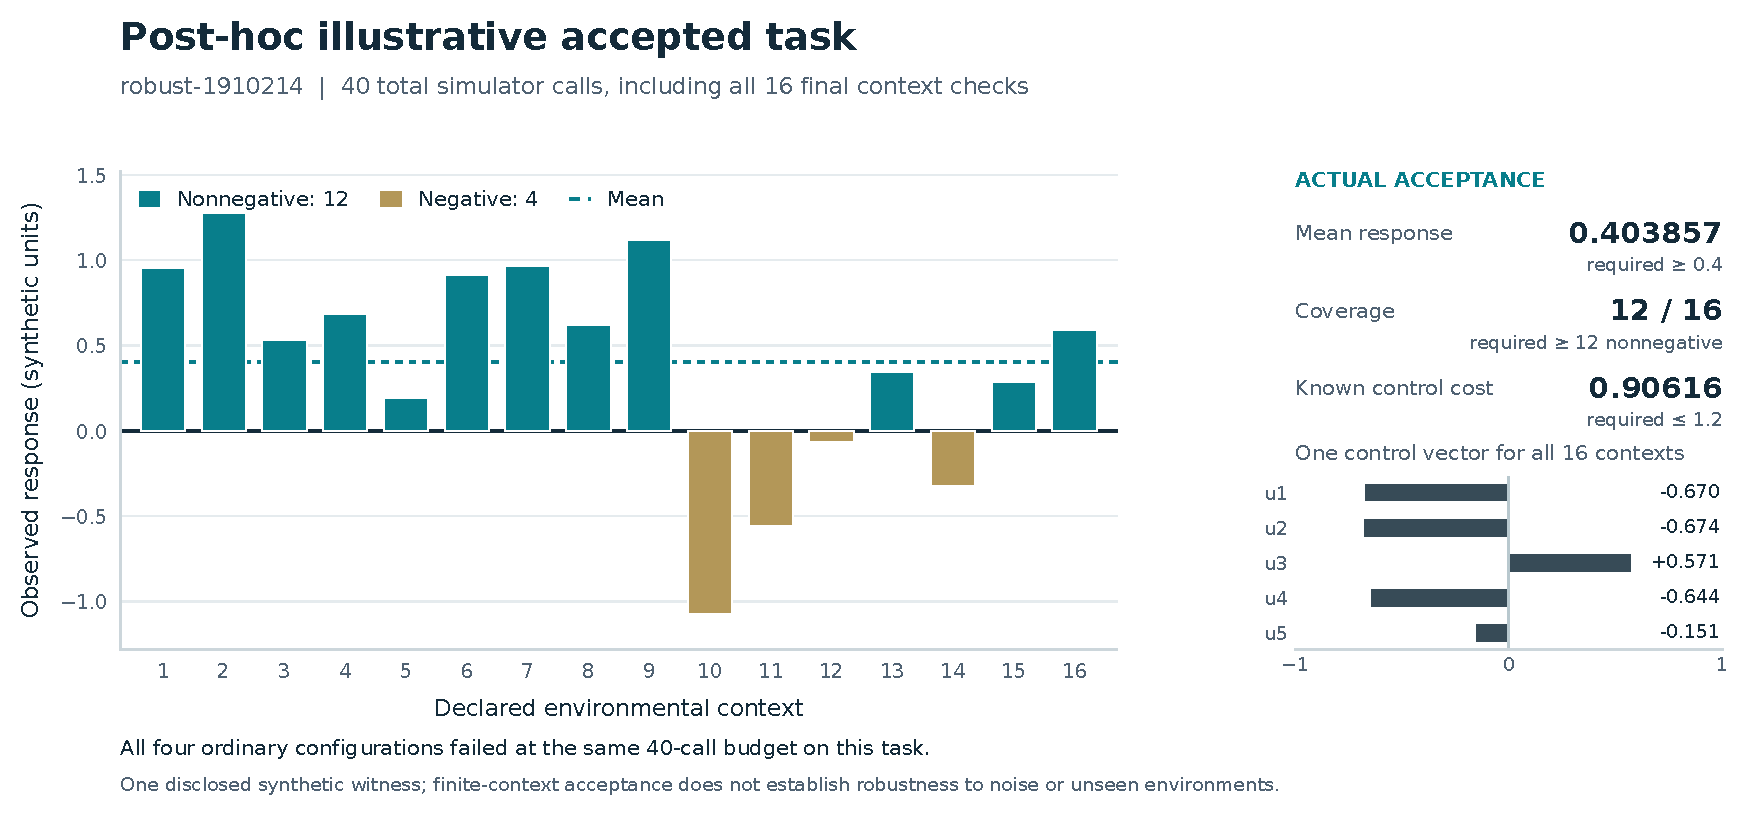
\includegraphics[width=\linewidth]{figures/witness.pdf}
\caption{An inspectable useful output. Each bar is a final actual simulator observation at the same control vector under one declared environment. The evidence certifies these sixteen deterministic contexts only.}
\end{figure}

The supplement prices this new scope only as a post-confirmation willingness-to-pay sensitivity; its technical contract was fixed before evaluation, but its price grid is not a preregistered buyer experiment. For example, at an assumed USD 100 per accepted plan, USD 0.10 per simulator call and twenty eligible reuses, the compatible stratum's mean per-attempt collected contribution is USD 44.78 for v2 versus USD 16.40 for direct search. The calculation includes failed delivery calls, all final checks, the assumed token/tool/service bundle, payment fees, invocation, USD 90 of shared lifecycle cost and the 1,280-call Gym amortized over the twenty hypothetical reuses. Both contributions are positive: this population average is improved conditional economics, not a claim that the baseline business is economically impossible. A specialist-only finite task crossing is a different statement from population-level reliability or a validated commercial offering.

These contributions also exclude the separately disclosed common opportunity-development research. The compound campaign used 617,544 query-equivalent evaluations, including fresh audit truth, all method comparisons and the illustrative replay. Pricing every unit at USD 0.10 would imply USD 61,754.40 of research expense before unmeasured engineering labor. Actual observed paid API expense and customer collections were zero. This burden exceeds the primary simulation's mean thirty-day operating profit and must be recovered separately before whole-study profitability can be claimed. The hypothetical tariff is not a bill for the inexpensive local synthetic computation, nor is local execution a reason to treat a future physical research campaign as free.

\section{Experiment C: capability-conditioned offering development}

Matched enterprises receive the same customer evidence and permission to select or prototype alternatives. The implemented proposal space is a finite, researcher-authored menu of response characterization, verified inverse design and a diagnosis prototype. Each policy uses development outcomes to choose among scopes and budgets, then freezes its proposal before fresh evaluation. Independent fresh outputs determine acceptance. A proposer cannot establish demand or price by describing its own proposal as valuable.

The matched policies select and prototype the diagnostic offering using the same evidence, but an ordinary paired-difference method identifies the single changed interaction in all 48 fresh cases with 32 observations. The retained model is therefore unnecessary for that synthetic diagnosis. The primary enterprise does not count diagnostic sales because field verification and willingness to pay are unestablished; only a separately named market-hypothesis scenario permits them. Prototype development remains charged. This failed additional-Alpha case is preserved alongside the positive compound-plan result rather than replaced by it.


This tests capability-conditioned \emph{selection and qualification} within a declared opportunity space. It does not establish autonomous, open-ended invention of a new business. The limitation is substantive: devising a scientifically valid new offering, finding a buyer and executing the first commercial engagement remain separate tasks. The useful contribution is the auditable lineage from earlier observations to a candidate service's fresh delivery, including a reason to reject an investment when an ordinary method or weak demand makes it unattractive.

The robust-plan extension adds a concrete example of researcher-assisted opportunity development: the initial task revealed that an accurate model was unnecessary for one satisfactory action; a compound mission then tested where a model could matter. The baseline received the same new brief and permission to bypass modeling. Its advantage is evaluated on new outputs rather than a proposer-assigned value score. Demand and willingness to pay for that compound offering remain unvalidated, so its hypothetical opportunity value is never booked as profit.

\section{Commercial accounting and enterprise decisions}

\subsection{Disjoint cost categories}

The ledger has three mutually exclusive cost classes. A contains complete paid-job delivery, including learning, per-job invocation, serving and validation required for that outcome. B contains additional assessment, retention, admission, distribution, maintenance and requalification not already charged to a delivered job. C contains optional Gym development and research beyond the paid outcome. The originating job's learning is charged once to A; the same observations are not billed again as Gym training. Rejected candidates and failed prototypes retain their cost.

\begin{center}\small\begin{tabular}{p{0.34\linewidth}p{0.58\linewidth}}
\toprule
Input & Primary specification \\ \midrule
Human service anchor & USD 80/hour (sourced list rate) \\
Estimated scopes & 12 hours model; 16 hours single-plan design \\
Selected primary quotes & USD 624 model; USD 832 verified design \\
Simulator tariff / latency & USD 0.10/call; 30 seconds/call (assumed) \\
Model/tool/service bundle & USD 9/job before queries/fees (assumed) \\
Horizon / arrivals & 30 days; 4 opportunities/day (assumed) \\
Resources & 3 agents, 8 hours/day each; USD 12,000 seed \\
Collections / reserve floor & 7-day delay; USD 2,000 minimum reserve \\
Replicates / scenarios & 64 matched seeds; 30 frozen scenarios \\
\bottomrule
\end{tabular}\end{center}
Every quantity in this table apart from the published rate is an assumption or a policy selection within that assumption set. Model token volumes are not API traces. The USD 9 bundle includes assumed frontier inference, tools, packaging and residual service costs; it imposes no arbitrary human-review minutes. Payment fees, failed deliveries, assessment, optional practice, obligations and reserves are added explicitly. Actual research engineering effort and its complete realized monetary cost remain unknown; native accounting preserves unknown cost fields rather than converting them to zero.


Cash expenses and displaced work are distinct. We report operating profit as recognized revenue less A, B and C expenses, and separately reconcile collections, receivables, unpaid obligations, seed capital, reserves and available cash. Additional work enabled by released capacity is counted only when the workload actually supplies an eligible job. Customer savings, token issuance, speculative opportunity value and seed funding are not earned revenue. The existing \$AGIALPHA mechanism is not used as a substitute for operating profit.

\subsection{Decisions with information available at the time}

Policies can deliver, assess, practice, invoke, share, develop an offering, preserve cash or stop. They use development estimates rather than confirmation answers to choose methods, prices and admission. The Beta-only, private and shared policies face the same event stream and initial resource limits. The shared policy pays its additional access and distribution costs. A second scenario may allow available surplus to finance capacity, but a gain from purchasing more capacity is reported as expansion, not evidence of intelligence compounding.

Independent review found a causal accounting defect before final reporting: the original replay checked capacity and cash against a direct search's future realized stopping cost. The corrected replay first reserves the declared maximum obligation, accesses the realized outcome only after admission, then releases unused resources. Preserved before/after boundary probes show that the original admitted unfundable or over-capacity work whereas the correction rejects it without reading protected outcomes. Original source and freeze, the correction amendment and unchanged development-selected policies remain available. Published economics use the corrected implementation.

\begin{center}\small\begin{tabular}{lrrrrr}
\toprule
Policy & Revenue & Cost & Profit & Collected & Available \\ \midrule
Beta only & 52,625 & 5,844 & 46,781 & 37,262 & 38,787 \\
Private selective & 50,360 & 5,972 & 44,388 & 34,997 & 36,507 \\
Shared selective & 50,360 & 5,972 & 44,388 & 34,997 & 36,507 \\
Controlled Gym pilot & 48,092 & 6,221 & 41,871 & 32,729 & 34,104 \\
\bottomrule
\end{tabular}\end{center}
All entries are mean simulated USD over 30 days. Beta's operating profit is 46,781.09, with conditional seed interval [45,409.91, 48,152.27]. Its A/B/C costs are 3,719.76, 2,051.60 and 72.80. Mean collections are 37,262.50; receivables are 15,362.75. Cash of 43,879.23 includes the separate 12,000 seed capital. Reserves are 4,631.26; unpaid obligations are 460.88. Available funds are 38,787.08; available earned surplus is 26,787.08. These distinct quantities reconcile in every retained run.

The primary optional policies reject v1 and preserve cash instead of choosing Gym training. They still pay for assessing the candidate and lose delivery capacity while doing so. Their mean profit is USD 2,393.30 below Beta. A controlled Gym-pilot arm deliberately pays for development so that the experiment can test v2; it is not the endogenous optimizer's selected action. That arm rejects v2 at the unrestricted envelope and loses USD 4,910.24 relative to Beta. Rejecting the investment does not erase the cost of discovering that it was unattractive.\par In the predeclared 40-call fitting-envelope scenario, the controlled Gym pilot has mean conditional profit USD 10,599.20, versus Beta's 6,160.18. Its paired increment is 4,439.01, interval [3,957.35, 4,920.68]. Response-model contracts still pay 384 additional acceptance queries in both arms. This narrow-envelope economic result is separate from the robust-plan supplement and from the primary 96-call scenario. The pilot uses a point-forecast investment rule; the existing lifecycle instead rejects the candidate under its conservative uncertainty rule. The pilot is a controlled counterfactual, not an authorized shared-production outcome passing that gate. It depends on assumed buyer behavior, scarcity, prices and reuse, and does not establish net value from sharing rather than private use.


\begin{figure}[H]
\centering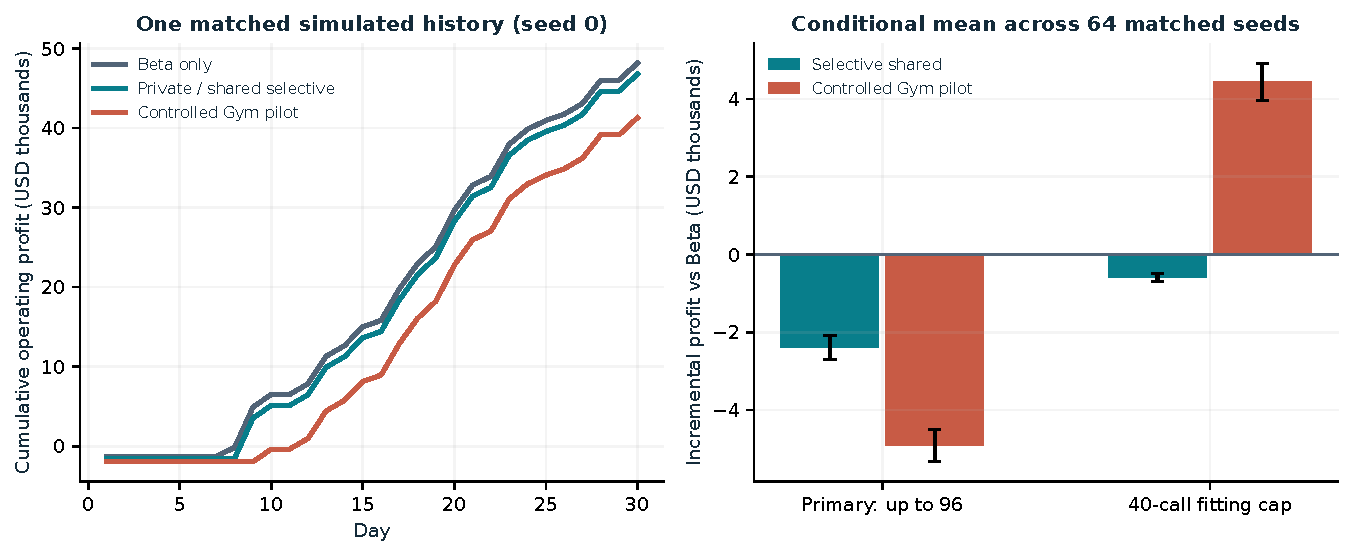
\includegraphics[width=\linewidth]{figures/economics.pdf}
\caption{Conditional enterprise outcomes. Curves are simulated cash/profit paths driven by measured technical outcomes and frozen economic assumptions. They are not customer receipts. Research costs and operating costs are both disclosed.}
\end{figure}

\subsection{Reconcile the research as well as the operating ledger}

The enterprise replay and the research campaign answer different accounting questions. The former includes each policy's required delivery, assessment and optional investment. The latter records what this edition actually evaluated to compare all those counterfactuals, including unsuccessful and duplicated development work. The primary confirmation alone consumes 90,172 method observations plus 44,544 common audit values; the audit-only number is not its full research cost. The following inventory makes the wider burden visible.

\begin{center}\small\begin{tabular}{lr}
\toprule
Recorded research phase & Query-equivalent units \\ \midrule
Original construction learning run & 11,396 \\
Final origin plus ten Gym jobs & 11,616 \\
First-task development smoke & 2,728 \\
Full 12-task development & 33,921 \\
Full 48-task confirmation & 134,716 \\
Robust 12-task development & 123,690 \\
Robust 48-task confirmation & 493,814 \\
Illustrative robust crossing replay & 40 \\
Recipient replay mission-fixture preparation & 39 \\
Separate protected integration recipient & 968 \\
Documented resource subtotal & 812,928 \\
\bottomrule
\end{tabular}\end{center}
This is a documented workload subtotal, not a certified complete research cost. It includes deliberate repeated construction and smoke campaigns. The original constructor's audit count is reconstructed from the executed routine rather than a separately preserved audit file. Common audit labels are counted once per task and campaign; literal recomputation of 8,576 already-known robust replay labels would raise the subtotal to 821,504. At the hypothetical USD 0.10 tariff, the two subtotals are USD 81,292.80 and USD 82,150.40. No corresponding invoice was incurred. Engineering effort, plotting, bootstrap, review and ordinary computing costs are unmetered. Paid-origin observations and the Gym already present in a policy's A/C ledger must not be charged again when allocating these study costs. This resource inventory does not justify subtracting the whole campaign mechanically from every simulated enterprise.


\subsection{When retention or sharing should stop}

For a homogeneous stream, a useful break-even approximation is
\[
N^{\star}=\frac{C_B+C_C}{\Delta m-c_{\rm serve}-c_{\rm upkeep}},
\]
provided the denominator is positive. Here $\Delta m$ is the additional collected contribution per eligible accepted job. If the denominator is nonpositive, more reuse does not repay the investment. In the actual simulation, heterogeneous outcomes, delays, failed deliveries, congestion and retirement replace this simple approximation.

The stress campaign varies demand, price, trust, simulator cost, serving capacity, delays, maintenance and obsolescence. Correlated validator error is a common-mode failure: repeating similarly mistaken checks does not create independent assurance. A stronger Beta that already contains the v2 information removes its information advantage, while retaining distribution and maintenance costs. This is a realistic retirement trigger, not evidence that the original learning never happened.

\begin{center}\small\begin{tabular}{lrrr}
\toprule
Scenario & Beta profit & Gym pilot profit & Pilot increment \\ \midrule
half demand & 22,641 & 19,724 & -2,916 \\
low trust & 8,922 & 7,439 & -1,482 \\
query price 0 5 & 666 & 666 & 0 \\
query price 2 & -102 & -102 & 0 \\
validator correlated & 46,758 & 41,849 & -4,909 \\
extra 896 verification & 23,321 & 20,492 & -2,829 \\
query envelope 40 & 6,160 & 10,599 & 4,439 \\
stronger beta & 44,407 & 40,160 & -4,247 \\
\bottomrule
\end{tabular}\end{center}
The USD 0.50 and USD 2 query cases make the assessment campaign unaffordable within the declared reserve constraint; the policy preserves cash after the originating job instead of assuming unlimited financing. Some stressors have no effect because the relevant skill was never admitted. That inactivity is informative and is not a successful stress test of a deployed sharing service. Correlated-error scenarios record mistaken invoices, refund obligations and unrecovered delivery/fee costs. Same-content library profit gaps are zero. Additional capacity is not purchased merely because funds exist when the frozen expansion condition is unmet. The confirmation research audit itself is disclosed separately as 44,544 unique oracle-equivalent observations, or USD 4,454.40 at the primary hypothetical tariff, rather than hidden as free acceptance or repeatedly charged to all enterprises.


\section{Protected sharing and existing-system integration}

The study does not create a competing registry. It reuses unchanged, hash-pinned lifecycle code from the existing research lane and the current native journal, trust and cost interfaces. The protected object is the effective machine-readable artifact. A prose summary is not treated as equivalent. Provenance includes the source commit, artifact digest, rights declaration, feature-library compatibility, resource needs, assessment evidence and limitations.

The recorded integration campaign passes 29/29 directed controls against 29 unchanged upstream files. It transports the actual 2,753-byte v2 artifact and checks identical retrieval, rights, current fixture membership, revocation, altered bytes, AES-GCM context binding, idempotency and disjoint costs. A separate recipient fits an unfamiliar task from the recovered bytes in 40 observations and delivers an accepted operating decision; the same-content ordinary library produces identical output. That recipient is an integration witness, not an additional independent confirmation sample.

The actual development-evidence admission assay rejects v2 at both tested 96-call and 40-call envelopes. At 96 calls its mean incremental per-use value is USD -6.85; at 40 its positive mean is too uncertain for the gate's conservative bound after assessment and lifecycle costs. Both corresponding production-like research retrievals remain denied. Positive access conformance uses explicitly artificial monetary evidence and never substitutes for an empirical admission. Real measured complete profit remains unknown in the native unknown-cost control.


Fixture identities exercise authorized access, revocation, rights checks, tamper rejection and retrieval of actual bytes. These are executable conformance results with simulated authority, not live chain authentication. Artificial positive evidence used solely to exercise a branch is kept distinct from the candidate's actual economic assessment. A denied candidate remains denied. The production capsule supports a bounded public-source-selection scope; this scientific artifact remains unsupported there. No successful research transfer widens execution permissions or bypasses existing Jobs validators, governance or settlement rules.

Three forms of sharing have different meanings. An executable skill may be copied and run with its prerequisites. A compatible trained component may be distributed only with appropriate rights and runtime support. A specialist service may be invoked without giving the recipient independent possession of its learned expertise. This edition transfers an empirical representation plus executable fitting code; it demonstrates neither a proprietary-model checkpoint transfer nor every agent becoming the same specialist.

\section{Frontier-model operating configuration}

Official model references checked on 27 October 2026 list \texttt{gpt-6-astra}, \texttt{gpt-6.1-sol} and \texttt{gpt-6.1-terra}. Their respective Standard input/output rates are \money{10}/\money{50}, \money{2}/\money{10} and \money{1}/\money{5} per million tokens; cached-input rates differ. Model pages document supported reasoning settings and tools; the source dossier records limits, caching and pricing modifiers \cite{astra,sol,terra,pricing}. These are provider observations, not measured account entitlements or the benchmark's actual token invoices.

A suitable live protocol would use Astra-class reasoning for problem formulation, experiment selection and independent review, and a capable tool/computer-use configuration for interacting with the actual scientific software. Both baseline and specialist receive the same contexts, tools, correction opportunities and total inference budget. Reasoning mode and effort, failure retries, search and execution environments are recorded. Model upgrades trigger a fresh baseline comparison. The present experiment uses no live frontier calls and makes no claim that its conventional portfolio exhausts frontier reasoning.

ChatGPT Pro is a subscription plan, not an API model identifier. Separately authorized access paths may exist, but entitlement, scopes, limits and costs must be checked for the actual application. The retrieved model pages do not support fine-tuning these proprietary weights, and the pricing documentation describes changes to fine-tuning availability. The economical intervention studied here is executable structure learning with ordinary numerical tools, not an assumed ability to edit provider weights.

\Needspace{10\baselineskip}
\section{Operating blueprint}

\subsection{Offer the verified outcome first}

The first offer should be a bounded scientific-software qualification engagement: obtain a customer's actual simulator, frozen acceptance requirements, permitted data and a plausible cost/latency profile; compare a capable conventional workflow with the retained representation; return an executable deliverable and a complete cost record. Quote against a matched human-service scope and buyer value. The sourced hourly anchor is a calibration input, not a reason to set every price at a fixed discount or close to production cost.

Choose production alone when competent Beta meets the contract profitably and learning adds insufficient expected value. Retain a private skill when reuse is credible and the artifact's causal benefit survives independent fresh cases. Share when recipients have compatible prerequisites, lawful access and enough net benefit after transfer and servicing. Use the Gym only when additional observations are likely to recover worthwhile missing structure. Stop or retire the artifact when ordinary methods catch up, incompatible tasks dominate or maintenance absorbs the gain.

\subsection{What could become feasible next}

If a customer's simulator family exhibits stable transferable structure and the learned representation materially reduces required observations, a smaller-budget or shorter-deadline response or design service becomes a testable opportunity. A maintenance diagnosis is attractive only if a conventional paired measurement or direct search cannot provide the same result more simply. Complementary specialists can then address different constraints: representation learning, experimental selection and independent output checking. Composition must improve the complete mission, not merely increase the number of invocations.

Live operation requires four specific additions: scope-matched customer evidence and willingness-to-pay tests; a real tool-using frontier baseline on the customer's software; observed simulator, validation and model invoices with collection/refund behavior; and current authority checks plus supported production execution scope. These are missing measurements rather than ceremonial approval steps. They should be acquired in a bounded pilot before scaling the service.

\subsection{Commercially sensible stopping rules}

Preserve operating reserves before optional investment. Do not spend solely to satisfy a prescribed reinvestment ratio or learning cadence. Price to expected customer value, quality and capacity while allowing rejection and deferral. Requalify after meaningful model or tool upgrades and retain unsuccessful comparisons. When the ordinary baseline becomes sufficient, delivering profitable work with no retained Alpha is a successful policy.

\section{Limits, reproducibility and provenance}

The study is strongest as a reproducible test of a narrow mechanism. Its task family deliberately contains recurring structure; that assumption must be checked in a real market. The simulator is deterministic and synthetic. The pool of offerings is bounded and researcher authored. Independent evaluation means fresh data and separate evaluation logic within the research implementation; it does not mean external replication or organizational independence. Statistical intervals across seeds remain conditional on these assumptions.

The apparent gain may shrink under noise, misspecified feature libraries, stronger sparse solvers, broader frontier-model invention, simpler direct solutions or expensive output validation. The unrelated-prior and shift arms test some of those risks but do not exhaust them. Neither exact artifact versioning nor successful protected retrieval establishes engineering correctness. No specialist ASI, autonomous economic self-acceleration, live authenticated network or earned profit is established here.

This edition tests one representation specialist and ordinary methods that can consume it. It does not establish the incremental value of composing multiple independently developed specialists. Ten Gym jobs build one successor artifact; they are not ten independently profitable investment cycles. The fresh recipient and new-offering lineage is real within the synthetic program, while long-run maintenance, repeated succession and capability-driven demand creation remain unmeasured.

The companion includes the protocol, source hashes, training and Gym ledgers, actual learned artifacts, all fresh result rows, frozen economic policies, all 11,520 per-run complete accounting summaries, six representative complete seed-zero event ledgers and deterministic replay, integration receipts, source dossier, original-source audit and reproduction commands. Failures and rejected investments are preserved. The browser demonstration shows the same recorded data and marks scenarios explicitly; it does not silently generate guaranteed learning benefits.

\textbf{AI assistance and authorship.} This paper carries the author line requested by Vincent Boucher, President of MONTREAL.AI. AI assistants conducted source retrieval, implementation, execution, internal review, analysis and drafting. The author line does not imply that the author personally ran every check. Software construction and scientific choices are disclosed as researcher authored; automated updates are distinguished from autonomous discovery. All new source is released under Apache-2.0, with original upstream licenses preserved.

\section{Conclusion}

The experiment establishes an executable form of experience-trained specialization: a learned interaction representation improves fresh response modeling and, in a separately frozen compound mission, enables more accepted outputs inside a small complete observation budget. It also establishes boundaries. Direct action search can bypass the need for an accurate model; ordinary paired measurements can defeat the proposed diagnostic advantage; unrelated recipients reduce transfer; a larger conventional budget can erase a crossing; and an ordinary library containing the same capability matches the protected research route.\par Commercial simulation is positive for competent delivery under the stated market assumptions. The primary policy declines retention and Gym investment, while a predeclared tighter-envelope pilot shows a conditional economic benefit from the developed representation. The real admission gate still rejects the candidate on uncertainty-adjusted development evidence. No sales, sustained compounding, graph-specific advantage or live frontier-model superiority is established. The next justified step is to test the compound-outcome mechanism on an actual customer's expensive simulator with observed validation costs and a capable live frontier baseline.


The strategic opportunity remains precise: useful work can reveal reusable structure that changes the cost or reliability of a later outcome. The commercial foundation is accepted delivery. Retention, practice, distribution and new-offering development are optional investments whose complete incremental value must be demonstrated. A persuasive flywheel narrative becomes evidence only when the outcome, inherited information, causal comparison and reconciled economics can all be inspected together.

\clearpage
\begin{thebibliography}{20}
\small
\bibitem{diaz} P. Diaz, A. Doostan and J. Hampton. Sparse Polynomial Chaos Expansions via Compressed Sensing and D-optimal Design. \emph{Computer Methods in Applied Mechanics and Engineering} 336, 640--666 (2018). \href{https://doi.org/10.1016/j.cma.2018.03.020}{doi:10.1016/j.cma.2018.03.020}. \url{https://arxiv.org/abs/1712.10131}.
\bibitem{tropp} scikit-learn developers. OrthogonalMatchingPursuit API and algorithm documentation. Accessed 27 October 2026. \url{https://scikit-learn.org/stable/modules/generated/sklearn.linear_model.OrthogonalMatchingPursuit.html}.
\bibitem{ard} scikit-learn developers. Linear models: automatic relevance determination. Accessed 27 October 2026. \url{https://scikit-learn.org/stable/modules/linear_model.html#automatic-relevance-determination-ard}.
\bibitem{sdsu} San Diego State University, Computational Science Research Center. Services and external consulting fee schedule. Accessed 27 October 2026. \url{https://www.csrc.sdsu.edu/services/}.
\bibitem{purdue} Purdue University, Rosen Center for Advanced Computing. Industry partnerships and consulting rates. Accessed 27 October 2026. \url{https://www.rcac.purdue.edu/industry}.
\bibitem{paratools} ParaTools. Consulting services and rates. Accessed 27 October 2026; no new effective date inferred. \url{https://www.paratools.com/consulting/}.
\bibitem{objective} Objective Experiments. DOE and MSA consulting services and rates. Accessed 27 October 2026. \url{https://objectiveexperiments.com/consulting/consulting/}.
\bibitem{astra} OpenAI. GPT-6 Astra model reference. Accessed 27 October 2026. \url{https://developers.openai.com/api/docs/models/gpt-6-astra}.
\bibitem{sol} OpenAI. GPT-6.1 Sol model reference. Accessed 27 October 2026. \url{https://developers.openai.com/api/docs/models/gpt-6.1-sol}.
\bibitem{terra} OpenAI. GPT-6.1 Terra model reference. Accessed 27 October 2026. \url{https://developers.openai.com/api/docs/models/gpt-6.1-terra}.
\bibitem{pricing} OpenAI. API pricing and reasoning guides. Accessed 27 October 2026. \url{https://developers.openai.com/api/docs/pricing}; \url{https://developers.openai.com/api/docs/guides/reasoning}.
\bibitem{ineffable} D. Silver / Ineffable Intelligence. A Note from Dave and mission statement, 15 January 2026. Accessed 27 October 2026. Research motivation only. \url{https://www.ineffable.ai/}.
\bibitem{repo} MONTREAL.AI. AGI-Alpha-Agent-v0, immutable starting source \path{80b345828f34fd8a6e592977dd17ef37141305f4}; study and foundation source map in the companion. \url{https://github.com/MontrealAI/AGI-Alpha-Agent-v0}.
\end{thebibliography}
\end{document}
